
\section{Information Extraction}
\label{sec1}

The IE framework will be introduced by example of processing the job descriptions. The Finite-State Transducer(FST) library, which is used as pattern matching tools, will be introduced as well.

In natural language, a single concept often has multiple expressions to represent it. For example, the simple concept bachelor's degree,  can be expressed in many ways in job descriptions, e.g. B.S., BA/BS, 4-years-degree, and so on. Table \ref{tab:multispelling} shows the words that if followed with word ``degree'' have the semantic value of ``bachelor's degree''.

\begin{table}[ht]
\caption{All words mean bachelors} % title of Table
\centering % used for centering table
\begin{tabular}{  | p{15cm} |  }
 \hline
 "Baccalaureate","bachelors", "bachelor" ,"B.S.", "B.S","BS","BA","BA/BS", "BABS", "BSBA", "B.A." ,"4-year","4-year", "4 year", "four year","college","Undergraduate" , "University" \\
  \hline
\end{tabular}
\label{tab:multispelling} % is used to refer this table in the text\section{Pipeline of Information Extraction}
\end{table}

To add labels to a sentence, we use regular expression over tokens. A regular expression over token transfer a patten to a Finite-State Transducer (FST), and every token of that will be transferred to an edge of FST. If we use all the expressions of a semantic value to create a pattern, the pattern will be very large, and there are too many states in the FST. For example, if we use some words in Table~\ref{tab:multispelling} to create the pattern of semantic value ``bachelor's degree'', the pattern will like below:
$$ (~Baccalaureate~\mid~bachelors~\mid~bachelor~~\mid~B.S~\mid~BS~\mid~BA~)~~degree $$
If all words in Table~\ref{tab:multispelling} are added to the pattern, the FST will have too many edges, and the matching process will be very slow because of the problem of combinatorial explosion.

To resolve this problem, we proposed an approach to use the patterns to match the \textit{labels} of the tokens, not the the original text. In the system, we don't care what words the sentences really use, but want to extract the semantic value of the tokens which match the pattern. The details of the approach is described below.

At first, we created two dictionaries, which are used to label the tokens. In the first dictionary, the keys are the tokens, like words in Table~\ref{tab:multispelling}, and the values are the symbols for semantic values, like ``BS-LEVEL'' for ``bachelor's degree'', or ``MS-LEVEL'' for ``master's degree''. The values of the the second dictionary are the ontology hypernym of their keys, like keys ``BS-LEVEL'' and  ``MS-LEVEL'' both have value ``DE-LEVEL'', which means that bachelor's degree and master's degree are both one kind of degree level. We show the dictionaries for degree information in Table~\ref{tab:semanticlabeling}. There are also some words in the dictionaries that have the same first layer and second layer labels, which is shown in Table~\ref{tab:morelabels}.

\begin{table}[ht]
\caption{Semantic Labeling } % title of Table
\centering % used for centering table
\small
\begin{tabular}{  | l | l | l |   }
 \hline
 Original Text & Layer 1 & Layer 2  \\
 \hline
   bachelors  &  \multirow{4}{*} ~BS-LEVEL   & \multirow{10}{*} ~DE-LEVEL  \\
 \cline{1-1}
   bachelor   &     &    \\
 \cline{1-1}
   B.S.       &     &    \\
 \cline{1-1}
   Baccalaureate    &     &    \\
 \cline{1-2}
   Master     &  \multirow{3}{*} ~MS-LEVEL   &    \\
 \cline{1-1}
   MS         &     &    \\
 \cline{1-1}
   M.S.       &     &    \\
 \cline{1-2}
   PhD        &  \multirow{3}{*} ~PHD-LEVEL      &    \\
 \cline{1-1}
 Ph.D         &     &    \\
 \cline{1-1}
  Doctorate   &     &    \\
 \hline

\end{tabular}
\label{tab:semanticlabeling} % is used to refer this table in the text\section{Pipeline of Information Extraction}
\end{table}



\begin{table}[ht]
\caption{More Labels} % title of Table
\centering % used for centering table
\small
\begin{tabular}{  | l | l | l |    }
 \hline
 "Be", "be", "is", "are", "was", "were", "am"    &  ~BE          & ~BE     \\
 \hline
 "a", "A", "an", "An", "The", "the"              &  ~DE          & ~DE    \\
 \hline
 "MBA", "BSCS", "BSEE", "MSCS"                   & \multirow{2}{*}~MAJOR-DEGREE &  \multirow{2}{*}  ~MAJOR-DEGREE  \\

 "MSEE", "MSCE","MPH"     &   &  \\
 \hline
  "practical experience" , "work experience" & \multirow{2}{*}~EXPERIENCE  & \multirow{2}{*} ~EXPERIENCE  \\
  "professional experience", "experience��    &              &       \\
 \hline
 "preferred", "required", "desired"     &  ~PREFER-VBD  & ~PREFER-VBD    \\
 \hline
 "a plus", "mandatory", "desirable"     &  ~PREFER-JJ   & ~PREFER-JJ      \\
 \hline
 "similar", "related", "Relevant"    &  \multirow{2}{*}~DEGREE-JJ   & \multirow{2}{*}~DEGREE-JJ    \\
 "equivalent", "based"              &               &              \\
 \hline
\end{tabular}
\label{tab:morelabels} % is used to refer this table in the text\section{Pipeline of Information Extraction}
\end{table}


With the two dictionaries, we can label the tokens with two layers. Table~\ref{tab:labeldsent} shows how the sentence ``Bachelors  degree  in computer science or information systems.'' is labeled.

\begin{table}[ht]
\caption{Labeled sentence } % title of Table
\centering % used for centering table
\small
\begin{tabular}{  | c | c | c | c | c |c | c |c | c | c |  }
 \hline
 layer 2 & DE-LEVEL   & DEGREE & IN & MAJOR            & OR & MAJOR  &.  \\
 \hline
 layer 1 &  BS-LEVEL   & DEGREE & IN & MAJOR-CS         & OR & MAJOR-INFO & .      \\
 \hline
   words & bachelors   & degree & in & computer science & or & information systems & .     \\
  \hline
\end{tabular}
\label{tab:labeldsent} % is used to refer this table in the text\section{Pipeline of Information Extraction}
\end{table}

The pattern ``DE-LEVEL DEGREE  IN   MAJOR  OR  MAJOR ''  can match the sentence above, and the output of the matching process is ``BS-LEVEL'' for bachelor's degree, ``MAJOR-CS'' and ``MAJOR-INFO'' for two majors mentioned in sentence. In our system, most patterns match the labels in second layer. With this approach, the size of the FST for the pattern will be minimized, so speed of matching process can be improved.


\subsection{Patterns for Matching}
\label{subsec1}

As we explained in section B, we mentioned matching tokens in the second layer to patterns we defined. To match the labels in sentences to our patterns, we proposed a library that support matching pattern over tokens. The difference between this library and traditional regular expression is that the basic unit to be matched is token, not character. Some patterns used to match degree phrases are in Table~\ref{tab:patterns}. The patterns looks like regular expression, but they use tokens as the basic units.

\begin{table}[ht]
\small
\caption{Patterns to match degree sentences} % title of Table
\centering % used for centering table
\begin{tabular}{  | l  |  }
 \hline
 DE-LEVEL,  DE-LEVEL, OR  DE-LEVEL DEGREE   \\
 DE-LEVEL DEGREE ( IN  $\vert$  OF ) DT MAJOR   \\
 MAJOR-DEGREE  ,  MAJOR-DEGREE OR MAJOR \\
 DE-LEVEL (, DE-LEVEL)* (OR DE-LEVEL)? BE? PERFER-VBD   \\
 \hline
\end{tabular}
\label{tab:patterns} % is used to refer this table in the text\section{Pipeline of Information Extraction}
\end{table}


\subsection{Pattern Matching Library}
\label{subsec1}

Finite-State Transducers~\cite{roche1997finite} have been used as a tool to match patterns and extract information for more than 20 years. This approach has been demonstrated to be very effective in extracting information from text like CIRCUS~\cite{lehnert1991university} and FASTUS~\cite{hobbs199713}.  In the widely used NLP toolkit GATE~\cite{cunningham2002framework}, the semantic tagger JAPE (Java Annotations Pattern Engine) could describe patterns that are used to match and annotate tokens. JAPE adopts a version of CPSL (Common Pattern  Specification Language)~\cite{appelt1998common}, which provides FST over annotations. Chang et al. presented cascaded regular expressions over tokens~\cite{chang2014tokensregex}, which proposed a cascaded pattern matching tool over token sequences.

After studying these tools, we found most of them to be powerful and complex, but not very flexible. One reason is that developers need to learn some Domain specific Languages (DSLs) like CPSL. The other reason is the extra effort and time required to integrate the pattern matching tool into the system. So here we proposed a more flexible and lightweight FST framework, which can do regular expression matching over labeled tokens. We give the definition of Finite-State Transducer here. A Finite-State Transducer is a 6-tuple $(\Sigma_1, \Sigma_2, Q, i, F, E)$ where:
\begin{itemize}
  \item $\Sigma_1$ is a finite alphabet, called the input alphabet.
  \item $\Sigma_2$ is a finite alphabet, called the output alphabet.
  \item Q is a finite set of states.
  \item $i \in Q$ is the initial state.
  \item $F \subset Q$ is the set of final states.
  \item $E \subset  Q  \times \Sigma_1^* \times \Sigma_2^* \times Q$ is the set of edges.
\end{itemize}


For example, the FST $T_{d3} = \left(     \{ 0, 1 \} ,  \{ 0, 1 \} , \{ 0, 1 , 2 \} ,  E_{d3} \right ) $ where $E_{d3} = $ \{ ( 0, 0, 0, 0 ),   ( 0, 1, 0, 1 ), ( 1, 0, 0, 2 ), ( 1, 1, 1, 0 ), ( 2, 1, 1, 2 ), ( 2, 0, 1, 1 ) \}  is shown in Figure~\ref{fig:fst}.


\begin{figure}[htbp]
  \centering
  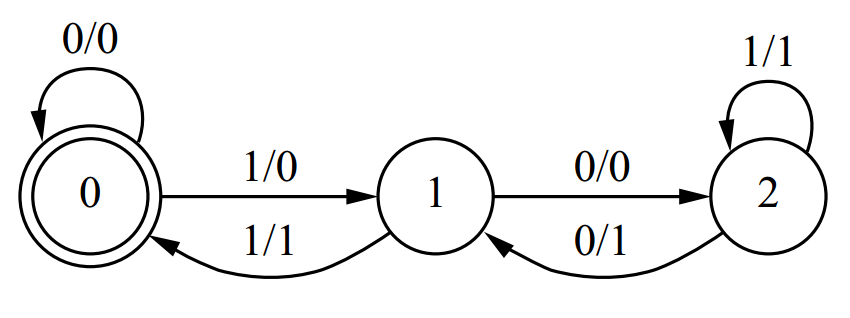
\includegraphics[scale=0.4]{images/fst.png}
  \caption{Zero or one NFA}
  \label{fig:fst}
\end{figure}

Regular expressions can be converted to automata \cite{aho1992foundations}, and FST is also an automata. To convert a regular expression over token to a FST we need two steps: The first is parsing the expression to a tree of matchers, the second is transfer the tree of matchers to the FST. We will introduce these two steps in next.

In our library, a ``matcher'' could be a token to be matched, or a composition of other matchers. Our library supports syntax used in traditional regular expressions over strings. We list the syntax that the library supports in Table~\ref{tab:matchers}. The first column is the names of the matchers, the second column is the explanation of the function of the matchers, and third column is the their counterpart syntaxes of traditional regular expression. The RegexMatcher in our library is constructed with a regular expression, and the matcher matches any string that matches the regular expression in the matcher. We give examples of the syntax of these matchers in Table \ref{tab:matchers_example}.

\begin{table}[ht]
\caption{Matchers of our Library } % title of Table
\centering % used for centering table
\begin{tabular}{  | l | l | l |  }
 \hline
 Matcher Name      &  Function                                 & Counter Part of regex    \\
 \hline
 UnitMatcher       &  token is matches the it                  & character  in regex       \\
 \hline
 SequenceMatcher   &  A list of Matcher                        & sequence of characters       \\
  \hline
 QuestionMatcher   &  One or more of the preceding token       & ?       \\
  \hline
 StarMatcher       &  Zero or more of the preceding token      & *       \\
  \hline
 PlusMatcher       &  Zero or one of the preceding token       & +       \\
  \hline
 DotMatcher        &  Any token                                & .      \\
  \hline
 RegexMatcher      &  Any token matches the regular expression               &  N/A      \\
  \hline
\end{tabular}
\label{tab:matchers} % is used to refer this table in the text\section{Pipeline of Information Extraction}
\end{table}



\begin{table}[ht]
\caption{Matchers' Examples } % title of Table
\centering % used for centering table
\begin{tabular}{  | l |  l |  }
 \hline
 Matcher Name          & Example    \\
 \hline
 UnitMatcher         & DEGREE       \\
 \hline
 SequenceMatcher     & DE-LEVEL DEGREE       \\
  \hline
 QuestionMatcher     & DE-LEVEL (OR DE-LEVEL)?  DEGREE       \\
  \hline
 StarMatcher         & DE-LEVEL (, DE-LEVEL)*  DEGREE       \\
  \hline
 PlusMatcher         & DEGREE IN MAJOR +      \\
  \hline
 DotMatcher          & HAS . DEGREE      \\
  \hline
 RegexMatcher        & r``d-d'' years  \\
  \hline

\end{tabular}
\label{tab:matchers_example} % is used to refer this table in the text\section{Pipeline of Information Extraction}
\end{table}

The framework supports three styles of creating patterns: regular expression style, operator style and object style. The second and third styles are flexible because developers can create their own matcher class to extend the feature of the library. We use examples to show how the three styles work. The most common style is defining pattern expression in a string, which is much like traditional regular expression.

\begin{framed}
\small
\noindent
The pattern is:  DE-LEVEL DEGREE ( IN  $\vert$  OF ) DT? MAJOR \\
The code is: \\
seqMatcher =parser.parse("DE-LEVEL DEGREE ( IN  $\vert$  OF ) DT? MAJOR")

\end{framed}

The second style is using algebraic operators to connect matchers, which can help developer reuse previous patterns when the new patterns include old ones. It is shown in follows:
\begin{framed}
\small
\noindent
The pattern is:  "DE-LEVEL DEGREE (IN $\vert$ OF) MAJOR" \\
The code is: \\
seqMatcher =  UnitMatcher("DE-LEVEL") +  UnitMatcher("DEGREE") + \\
\hspace{3cm} ( UnitMatcher("IN") $\vert$ UnitMatcher("OF" ) ) + UnitMatcher("MAJOR")

\end{framed}

We also could create a complex matcher in object-oriented programming style.

\begin{framed}
\small
\noindent
The pattern is:  "DE-LEVEL DEGREE (IN $\vert$ OF) MAJOR" \\
The code is: \\
matcher1 = UnitMatcher("DE-LEVEL") \\
matcher2 = UnitMatcher("DEGREE")  \\
matcher3 = UnitMatcher("IN")   \\
matcher4 = UnitMatcher("OF")   \\
matcher5 = UnitMatcher("MAJOR")  \\
matcher6 = AlternateMatcher([matcher3,matcher4])   \\
seqMatcher = SeqMatcher([matcher1, matcher2, matcher6, matcher5])

\end{framed}

The flexibility of the tool also comes from the fact that developers can determine which layer of the array should be matched, the original text, or labels in the first layer or labels in the second layer. Developers can assign a lambda expression to the matcher's catching function, which defines how to get the matching input strings from the sentences, as well as an out function, which defines what should be outputed. For example,  the labeled sentence is a sequence of arrays, each array includes the original text token and its labels in the other two layers, which is shown in table~\ref{tab:labeldsent}. To match the labeled sentence, we set the lambda expression for catching function to ``lambda x:x[2]'', and the out function to ``lambda x:x[1]'', which make the matcher match the label in second layer, and output the the value of semantic value in the first layer.

\subsection{Evaluation}

To evaluate the performance of the information extraction module, we extract sentence types through the use of sentence filters. To explain the process of our experiment, we use the sentences whose content pertains to the applicant's college degree information.

In the experiment, we selected 100 sentences from existing job descriptions, and the content of these sentences were requirements of candidate degree and major. We labeled the values for "degree" and "major" manually. We use some content patterns that we can identify from these sentences to match and extract the degree information. When we used 6 patterns, the accuracy of "degree" became 94\%. We also compared our pattern matching method to the conditional random fields (CRFs) model~\cite{lafferty2001conditional}, which is a state of art machine learning model for sequence labeling. We used 200 labelled sentences to train the CRF model, and the features of the CRF model are words in the sentences and part of speech tags of the words. The accuracies of information extraction of the three fields with our two methods, pattern matching, and the application of the CRF model are shown in Table \ref{tab:ieaccura}.


\begin{table}[ht]
\caption{Information Extraction} % title of Table
\centering % used for centering table
\begin{tabular}{   | c | c | c | c |   }
 \hline
          Field   & Pattern Num & Accuracy of Pattern Matching  & Accuracy of CRF   \\
 \hline
          Degree  & 6           & 0.94       &  0.85  \\
 \hline
          Major   & 10          & 0.85       &  0.72  \\
 \hline

\end{tabular}
\label{tab:ieaccura} % is used to refer this table in the text
\\Our pattern matching approach can get higher accuracy.
\end{table}